\section{Auswertung}
\label{sec:Auswertung}

\begin{table}
    \centering
    \begin{tabular}{
    S[table-format=3.0]
    S[table-format=1.2]
    S[table-format=1.2]
  }
    \toprule
    {Phase\;$\phi \left[\unit{°}\right]$} & {$U_{out}\left[\unit{V}\right]$} & {$U_{out noise}\left[\unit{V}\right]$}\\
    \midrule
    000 & 0.00  & 0.00 \\
    030 & 2.08  & 2.02 \\
    060 & 4.60  & 4.53 \\
    090 & 5.15  & 5.00 \\
    120 & 4.75  & 4.60 \\
    150 & 2.43  & 2.18 \\
    180 & 0.00  & 0.00 \\ 
    210 & -2.03 & -1.80  \\
    240 & -4.80 & -4.30  \\
    270 & -5.40 & -4.85  \\
    300 & -4.98 & -4.40  \\
    330 & -2.40 & -2.01  \\
    360 & 0.00  & 0.00 \\
    \bottomrule
\end{tabular}
\end{table}
In den Abbildungen 5 bis 9 sind Screenshots von der Anzeige des Oszilloskops für die verschiedenen Phasen $\phi$ dargestellt. In Abbildung 10 ist
die Anzeige bei Phase $\phi = 0$, jedoch mit aktiviertem Noise, dargestellt. 
\begin{figure}
    \begin{minipage}[b]{.45\linewidth} % [b] => Ausrichtung an \caption
       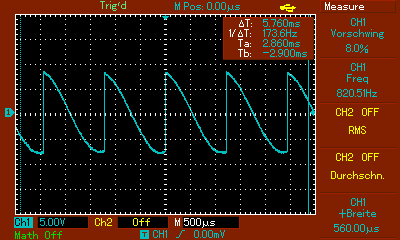
\includegraphics[width=\linewidth]{bilder/MAP003.png}
       \caption{$\phi = 0\,\unit{°}$}
    \end{minipage}
    \hspace{0.1\linewidth}% Abstand zwischen Bilder
    \begin{minipage}[b]{.45\linewidth} % [b] => Ausrichtung an \caption
       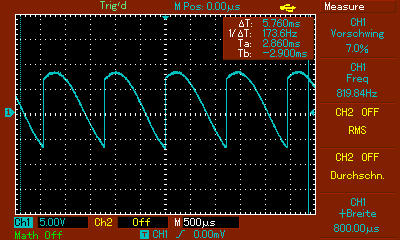
\includegraphics[width=\linewidth]{bilder/MAP004.png}
       \caption{$\phi = 30\,\unit{°}$}
    \end{minipage}
\end{figure}

\begin{figure}
    \begin{minipage}[b]{.45\linewidth} % [b] => Ausrichtung an \caption
       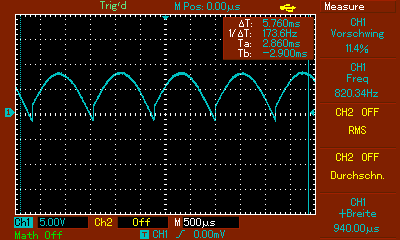
\includegraphics[width=\linewidth]{bilder/MAP005.png}
       \caption{$\phi = 60\,\unit{°}$}
    \end{minipage}
    \hspace{0.1\linewidth}% Abstand zwischen Bilder
    \begin{minipage}[b]{.45\linewidth} % [b] => Ausrichtung an \caption
       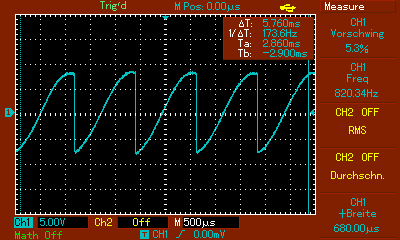
\includegraphics[width=\linewidth]{bilder/MAP006.png}
       \caption{$\phi = 90\,\unit{°}$}
    \end{minipage}
\end{figure}

\begin{figure}
    \begin{minipage}[b]{.45\linewidth} % [b] => Ausrichtung an \caption
       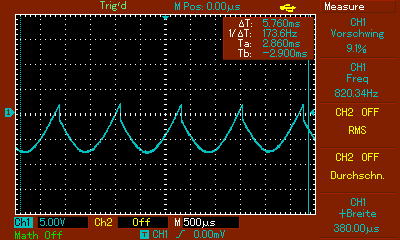
\includegraphics[width=\linewidth]{bilder/MAP007.png}
       \caption{$\phi = 120\,\unit{°}$}
    \end{minipage}
    \hspace{0.1\linewidth}% Abstand zwischen Bilder
    \begin{minipage}[b]{.45\linewidth} % [b] => Ausrichtung an \caption
       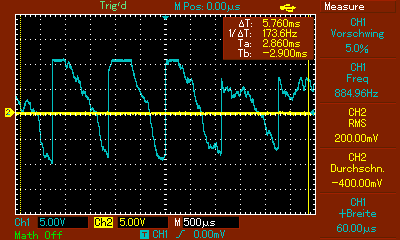
\includegraphics[width=\linewidth]{bilder/MAP011.png}
       \caption{$\phi = 0\,\unit{°}$ mit Noise}
    \end{minipage}
\end{figure}